% -*- mode: LaTeX; tex-main-file: "../Notes.tex"; -*-
% (begin: insert file SpectralEstimation.tex)
\section{Practical Considerations}
\label{sec:practical}
\ifthenelse{\boolean{nofootnotes}}
{\subsection{Windowed Fourier Transform}}
{\subsection{Windowed Fourier Transform\protect\footnotemark}
\footnotetext{Much of this subsection follows the presentation of
Sethares~\cite{Sethares:1997} p.288.}}
If there is only a single partial in the sound, then the spectrum
contains only this one partial.  In an ideal setting, the spectrum of
a pure sine wave is zero everywhere except at the frequency of the
sine wave.  However, in practice the FFT of a sine wave is not exactly
zero at points other than the true frequency, and there are two
different kinds of errors: roundoff  (numerical) errors and artifacts
(``edge effects''), that cause the representation of a sine wave to
``leak'' or ``smear out'' to other frequencies.

To give an example, let $T$ be the period (seconds per cycle) of the
sine wave. That is, it takes $T$ seconds to complete one full
cycle. Therefore, the wave has frequency $f=1/T$ cycles per second 
(Hz). Also, there are $2\pi$ radians per cycle, so the wave 
has frequency $\omega = 2\pi f$ radians per second.
Suppose that $f=220$ Hz and the sample rate is $SR=44,\!100$ samples per
second.  Define the \emph{normalized frequency} by
\[
 f_n = \frac{f}{SR}= \frac{220}{44100} = 0.005
\]
and suppose we sample the sine wave at a total of $N=2^{15}$
%=32,\!768 
points.  This provides $N/SR \approx 0.743$ seconds of sample data,
during which time the wave completes 
\[
   f \times \frac{N}{SR}  =  f_n \times N \approx 163.47 
\]
cycles.  Using these observations, and computing the Fourier transform
produces figure \ref{fig:FTaperiodic}.
The peak in the bottom graph correctly indicates that the true
frequency is somewhere around 220 Hz, but it is not very precise.  
The Matlab programs used to generate these figures are given in the
appendix at section~\ref{sec:Sinewave}. 

Given a periodic signal, the Fourier transform assumes that the entire
set of observations represents an integer number of periods for that
signal.  When this assumption is valid, concatenating the signal with
multiple copies of itself does not introduce any spurious
periodicities into the signal.  As shown in the top graph of 
figure~\ref{fig:FTaperiodic}, this assumption is not always valid.
Since the interval over which we sample the signal did not allow for
the completion of an integer number of periods, the concatenation --
depicted by the dashed extention in the figure -- gives a description
of the wave as something other than a pure sinusoid.
\begin{figure}
\ifthenelse{\boolean{nofigures}}{}{
%             \pdfimage
%             width 88 mm 
%             height 60 mm
%             {\HOME/figures/FTaperiodic.png}
\centering  
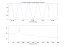
\includegraphics[width=120mm, height=70mm]{\HOME/figures/FTaperiodic}
}
\caption{{\small (top) The last four periods of a 220 Hz sine wave sampled
over the interval 0 to 0.743 seconds.  Since the wave can only
complete 163.47 cycles over this time interval, a concatenation of the
waveform (employed by the FFT and depicted by the dashed continuation
at $t=0.743$) introduces spurious frequency components into the signal.}}
\label{fig:FTaperiodic}
\end{figure}

Contrast the foregoing with what happens when the number of
observations in our sample set allows for an integral number
of periods.  This is easily accomplished when we are free to choose
all experimental parameters.  Suppose given are the sample rate, $SR =
44100$, and the number of observations $N=32768$, and suppose also that
we merely require the wave closely approximate the given frequency 
$f = 220$ Hz.  Then let   
\[
\tilde{f} = (SR/N)\lfloor (N/SR)f\rfloor \approx 219.37
\] 
The second factor, resulting from the ``floor'' operator $\lfloor \cdot
\rfloor$, represents the largest integer no greater than the number of
periods (163.47) completed by a 220 Hz wave during a sample time of
$N/SR$ seconds. 
As shown in Figure~\ref{fig:FTperiodic}, a concatenation of the
waveform -- depicted by the dashed continuation
at $t=0.743$ -- introduces no spurious frequency components.
\begin{figure}
\ifthenelse{\boolean{nofigures}}{}{
%             \pdfimage
%             width 88 mm 
%             height 60 mm
%%             width 13 cm
%%             height 10 cm
%             {\HOME/figures/FTperiodic.png}
\centering  
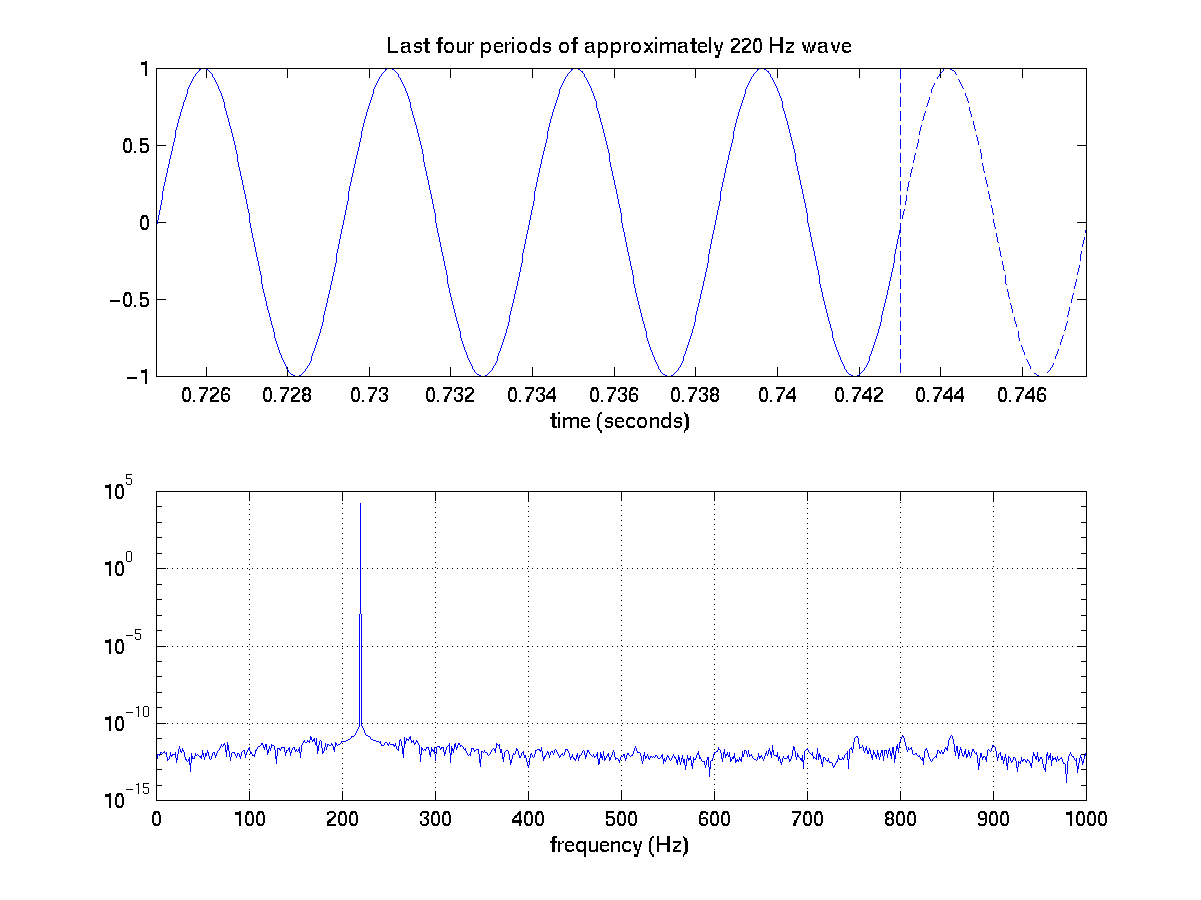
\includegraphics[width=120mm, height=70mm]{\HOME/figures/FTperiodic}
}
\caption{{\small (top) The last four periods of a 219.37 Hz sine wave sampled
over the interval 0 to 0.743 seconds.  Since the wave completes
exactly 163 cycles over this time interval, a concatenation of the
waveform (employed by the FFT and depicted by the dashed continuation
at $t=0.743$) introduces no spurious frequency components.}}
\label{fig:FTperiodic}
\end{figure}

From a practical point of view, it is natural to question the
utility of a method that depends on our ability to specify the
frequencies of the signals under study.
Instead, suppose we accept the signal frequencies as given and simply
adjust the number of samples used in the FFT to match the periods of
the existing frequencies.  Unfortunately, this is also impractical
when analyzing real sounds.  For, choosing this length
requires knowing the frequencies of the partials, and finding these
frequencies is precisely the FFT's raison d'\^{e}tre.

The problem -- exposed in Figure~\ref{fig:FTaperiodic} -- occurs because
the (empirical) ends of the signal don't line up; abrupt changes in
the waveform cause the spectrum to smear.  One way to force the ends
to line up is to preprocess the data so that it dies away to zero at
both ends.  Then, no matter what the underlying periodicity, there
will be no abrupt changes in the wave shape.

One popular approach is the \emph{Hamming} 
window\footnote{Named after Richard Hamming, this is a single cycle of
a scaled and shifted cosine wave.  The formula is $h(t) = 0.54 - 0.46
\cos(2\pi t/(N-1))$ for $0 \leq t < N$.  The Matlab code implementing
this technique is given in the appendix at section~\ref{sec:Sinewave}}.
The effect of the window on a 20 Hz wave is shown in
Figure~\ref{fig:hamming}.  The result of applying the window to a 220
Hz wave and then taking an $N$-point fast Fourier transform is
shown in Figure~\ref{fig:FThamming}. 
\begin{figure}
  \ifthenelse{\boolean{nofigures}}{}{
  \centering  
  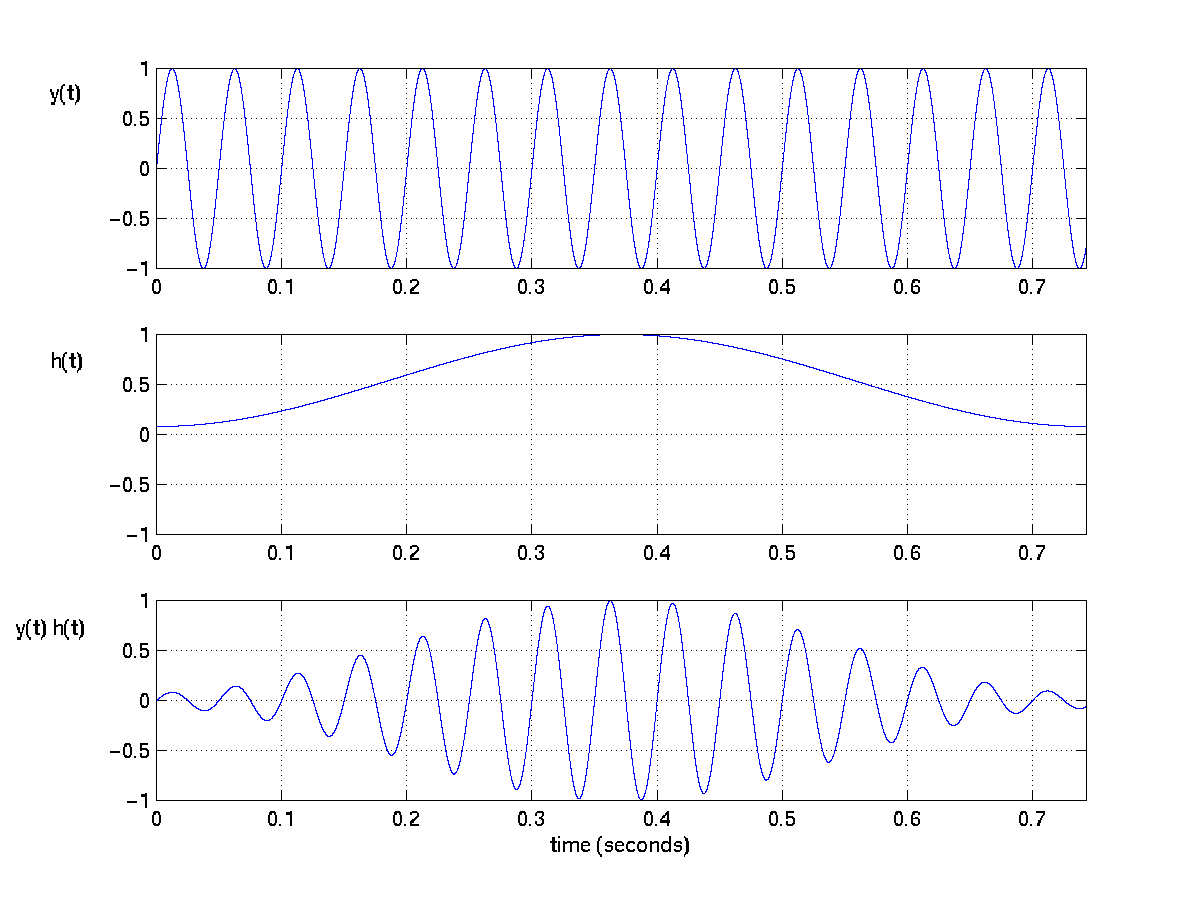
\includegraphics[width=120mm, height=70mm]{\HOME/figures/hamming}
  }
  \caption{{\small A 20 Hz sine wave (top) and a Hamming window (middle) are
  multiplied to produce the attenuated sine wave (bottom).}}
  \label{fig:hamming}
%\end{figure}
%
%\begin{figure}
  \ifthenelse{\boolean{nofigures}}{}{
  \centering  
  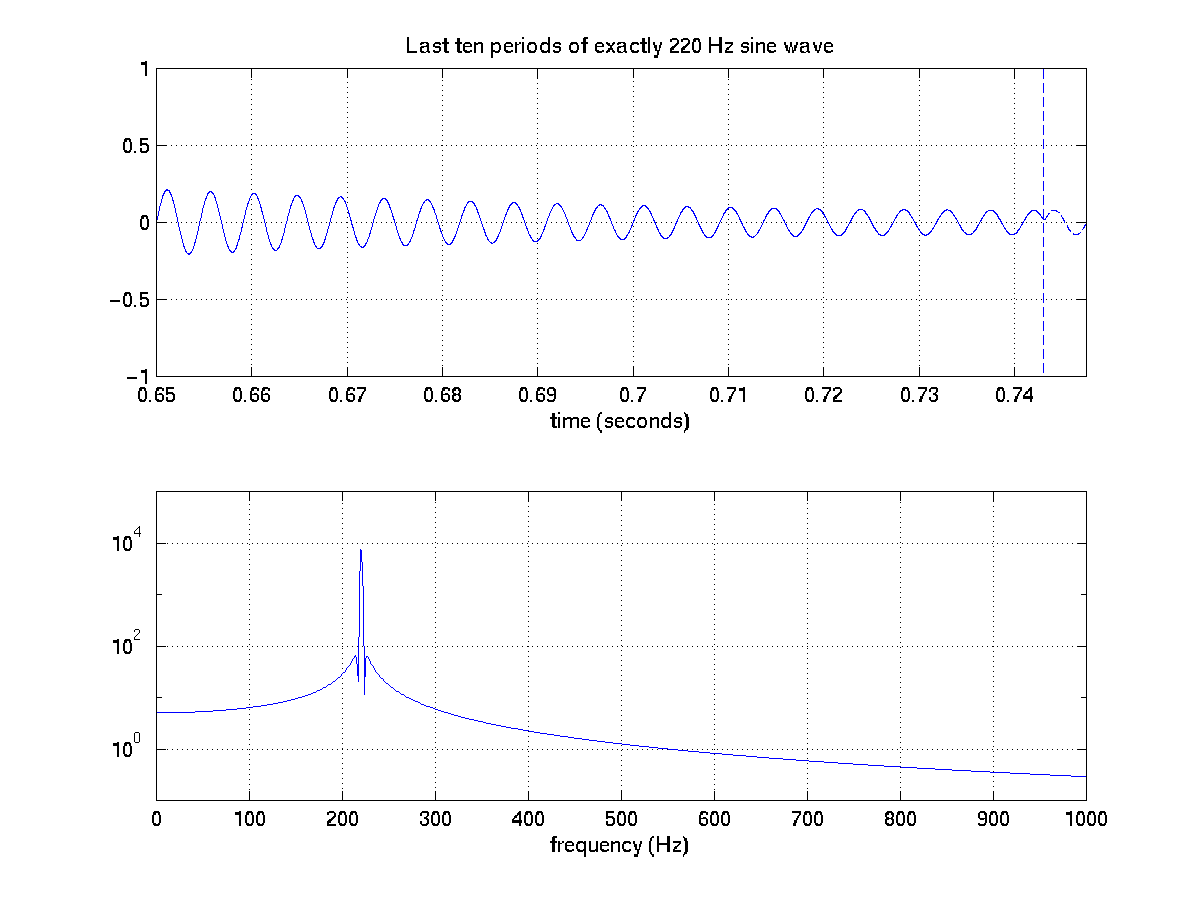
\includegraphics[width=120mm, height=70mm]{\HOME/figures/FThamming}
  }
  \caption{{\small (top) The last 10 periods of a 220 Hz windowed sine wave
  sampled over the interval 0 to 0.743 seconds.  Although the wave does
  not complete an integral number of periods over this time interval, a
  concatenation of the  waveform introduces less error than before
  because the wave is attenuated significantly at the point of
  aperiodicity ($t=0.743$).}}
  \label{fig:FThamming}
\end{figure}

The second cause of error when estimating the spectrum of a signal
concerns time versus frequency resolution.  The FFT measures the
frequency content of a signal on a given time interval, of length
$\Delta t$, over which we assume that the signal is approximately
stationary.  For real world signals, such as music, the approximation
gets worse as $\Delta t$ increases.  That is, the time intervals over
which we assume a constant frequency content must be small.
Precision in determining \emph{when} various frequencies
occur is the result of good or high \emph{time resolution}.

On the other hand, as the time resolution increases, the \emph{frequency
resolution} decreases.  This trade-off, a result of the well-known
\emph{uncertainty principle}, is illustrated by the following
scenario.  Assume a sample rate of $SR = 44100$ observations per second,
and a $4096$-point \emph{analysis window} (the interval over which to
compute the FFT).  This implies that each window examines $\Delta t =
N/SR \approx 0.093$ seconds of the signal.  In this case, the FFT measures
the frequency content of the signal by providing an $N$-element
vector of magnitudes indicating strength of spectral components at
(roughly) the frequencies {10.8 Hz, 21.5 Hz, \ldots, 44100 Hz}. The
general term in this sequence of frequencies is 
\[ 
k\times \frac{SR}{N} = k \times \frac{44100}{4096} 
		\approx k \times 10.77\text{ Hz,}
		\qquad  k\in\{1,2,\ldots, N\}
\] 
As shown by the top graph in Figure~\ref{fig:FFTbincomp}, the
frequency resolution is poor. 

Compare this to the same analysis at a lower time resolution, say
$\Delta t \approx 0.372$, obtained by setting $N= 16384$. This
provides the much clearer picture of the frequency content in the
bottom graph of Figure~\ref{fig:FFTbincomp}.  Still, the FFT only
indicates magnitudes at frequencies that are integer multiples of
$SR/N \approx 2.69$.  The presence in the signal of any frequency
components that \emph{are not} multiples of 2.69 (e.g.~220) is indicated by an
interpolation of the magnitudes at neighboring points (e.g.~218.0 and
220.7) which \emph{are} multiples of 2.69.
\begin{figure}
  \ifthenelse{\boolean{nofigures}}{}{
    \centering  
    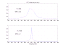
\includegraphics[width=120mm, height=70mm]{\HOME/figures/FFTbincomp}
  }
  \caption{{\small (top) The FFT of a 220 Hz windowed sine wave sampled over the
  interval 0 to 0.093 seconds. (bottom) The FFT of a 220 Hz windowed
  sine wave sampled over the interval 0 to  0.372 seconds.}  }
  \label{fig:FFTbincomp}
  %\end{figure}
  
  %\begin{figure}
  \ifthenelse{\boolean{nofigures}}{}{
    \centering  
    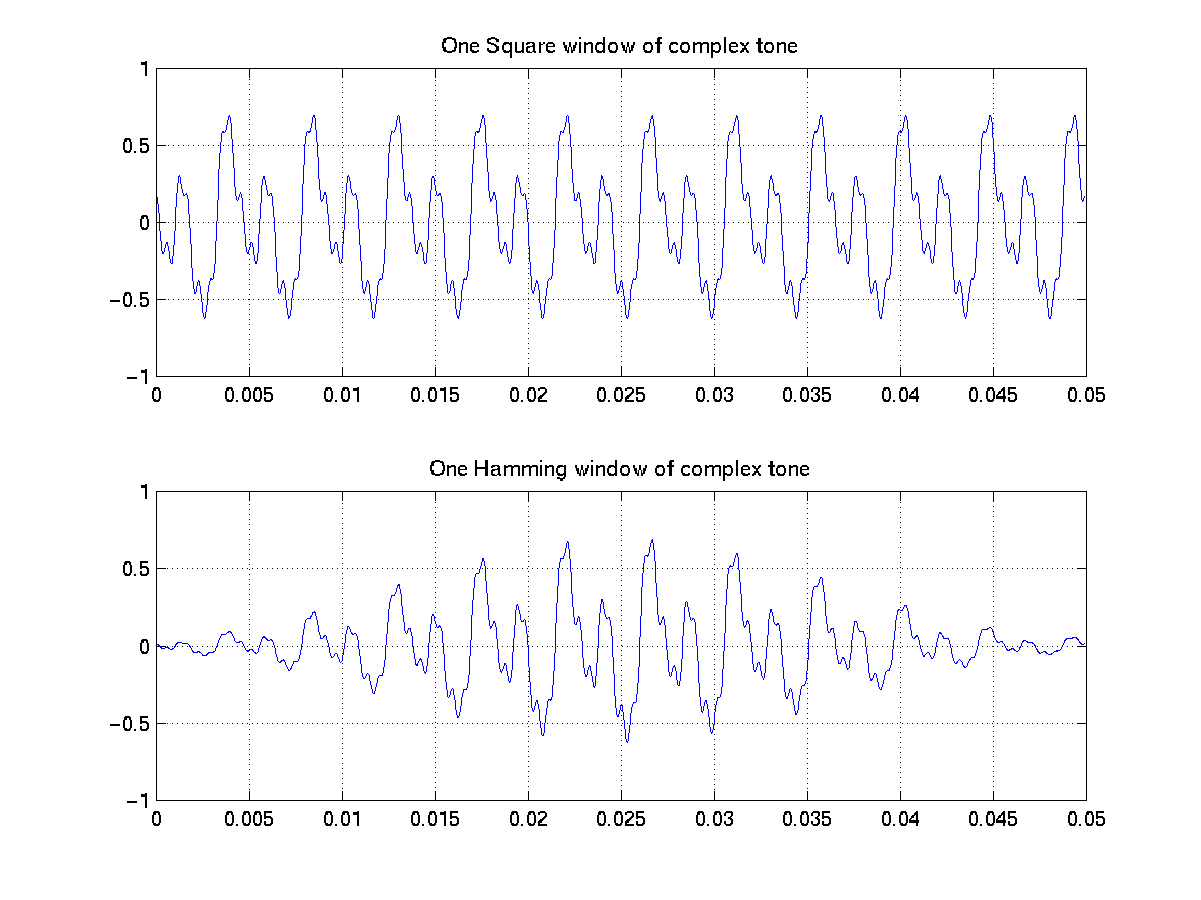
\includegraphics[width=120mm, height=70mm]{\HOME/figures/CompTone2200}
  }
  \caption{{\small A complex tone with frequencies 220, 440, 880, 1760 Hz and
  amplitudes .3, .4, .1, .1 (resp.) in a square window (top) and Hamming
  window (bottom) each of length 0.05 seconds.} }
  \label{fig:CompTone2200}
\end{figure}
  
\begin{figure}
  \ifthenelse{\boolean{nofigures}}{}{
    \centering  
    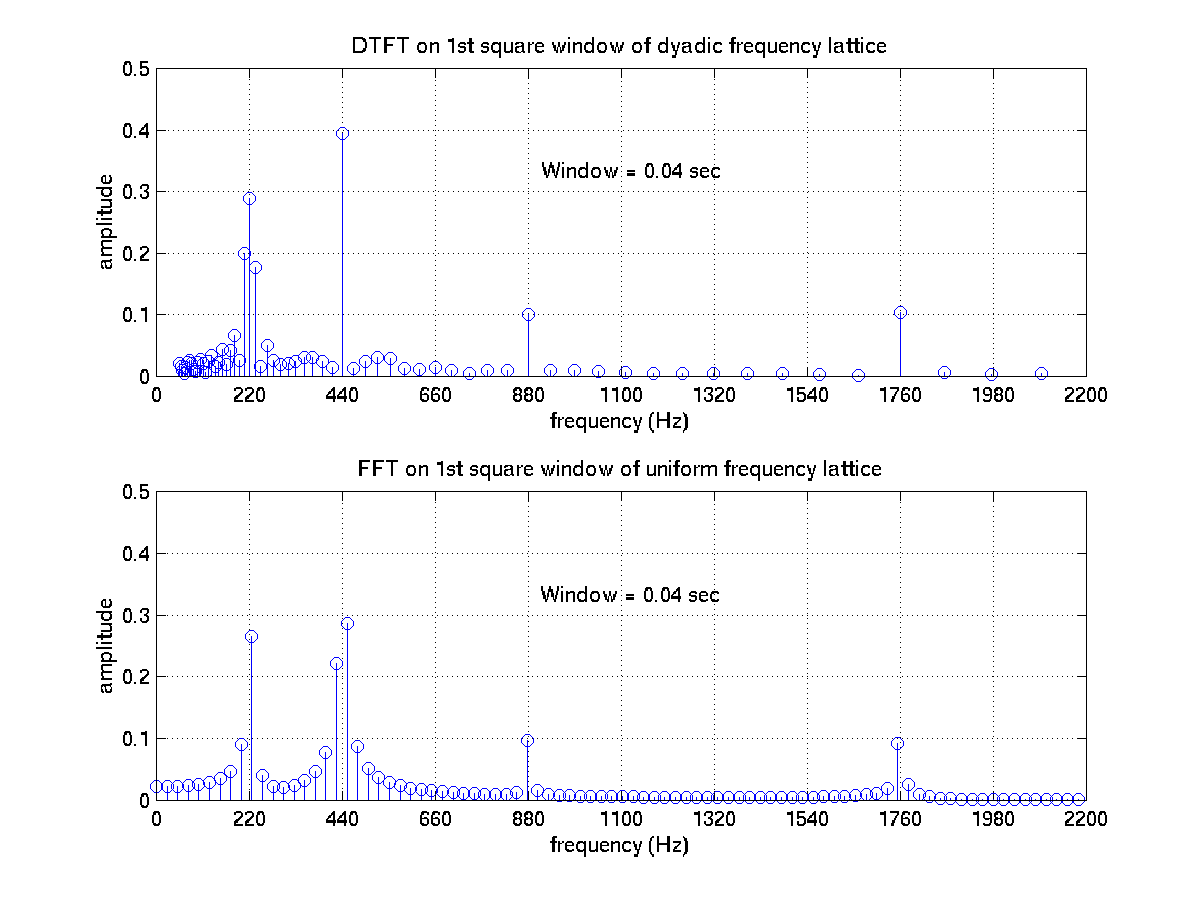
\includegraphics[width=120mm, height=70mm]{\HOME/figures/DTFTvFFTSq1760}
  }
  \caption{{\small The DTFT (top) and FFT (bottom) of a complex tone with
  frequencies 220, 440, 880, 1760 Hz and amplitudes .3, .4, .1, .1,
  (resp.) in a square window of length 0.04 seconds.}}
  \label{fig:DTFTvFFTSq1760}
  %\end{figure}
  
  %\begin{figure}
  \ifthenelse{\boolean{nofigures}}{}{
    \centering  
    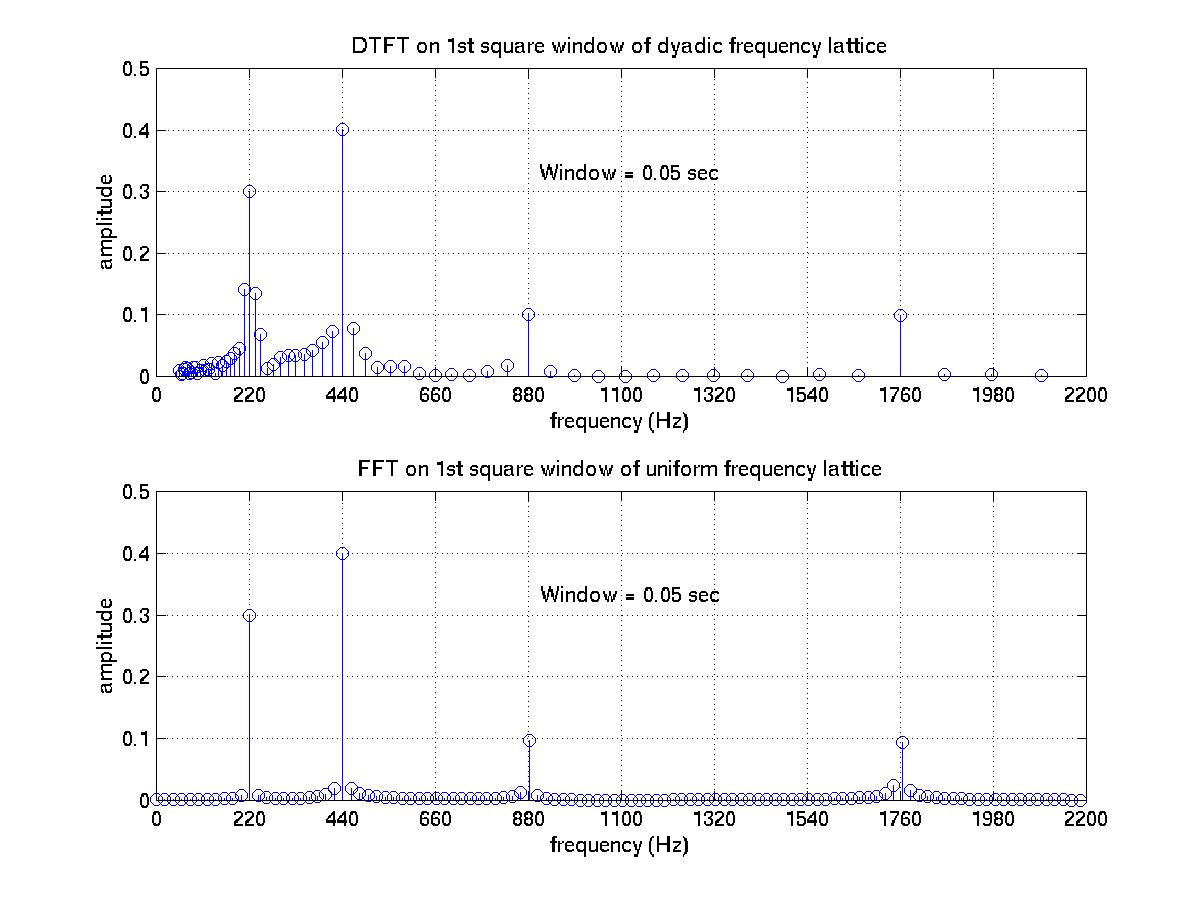
\includegraphics[width=120mm, height=70mm]{\HOME/figures/DTFTvFFTSq2200}
  }
  \caption{{\small The DTFT (top) and FFT (bottom) of a complex tone with
  frequencies 220, 440, 880, 1760 Hz and amplitudes .3, .4, .1, .1
  (resp.) in a square window of length 0.05 seconds.}}
  \label{fig:DTFTvFFTSq2200}
\end{figure}
%\begin{figure}
%             \pdfimage
%             width 13 cm
%%%             height 10 cm
%             {\HOME/figures/SpecDTFTHam1760.png}
%\caption{{\small The DTFT on a dyadic frequency lattice of a complex tone with
%frequencies 440, 880, 1320, 1760, 2200 Hz and amplitudes that start at .3, .4, .1, .1, .08,
%(resp.), decaying exponentially.}}
%\label{fig:SpecDTFTHam1760}
%
%             \pdfimage
%             width 13 cm
%%%             height 10 cm
%             {\HOME/figures/SpecFFTHam1760.png}
%\caption{{\small The FFT of a complex tone with frequencies 440, 880,
%1320, 1760, 2200 Hz and amplitudes that start at .3, .4, .1, .1, .08,
%(resp.), decaying exponentially.}}
%\label{fig:SpecFFTHam1760}
%\end{figure}
\begin{figure}
  \ifthenelse{\boolean{nofigures}}{}{
    \centering  
    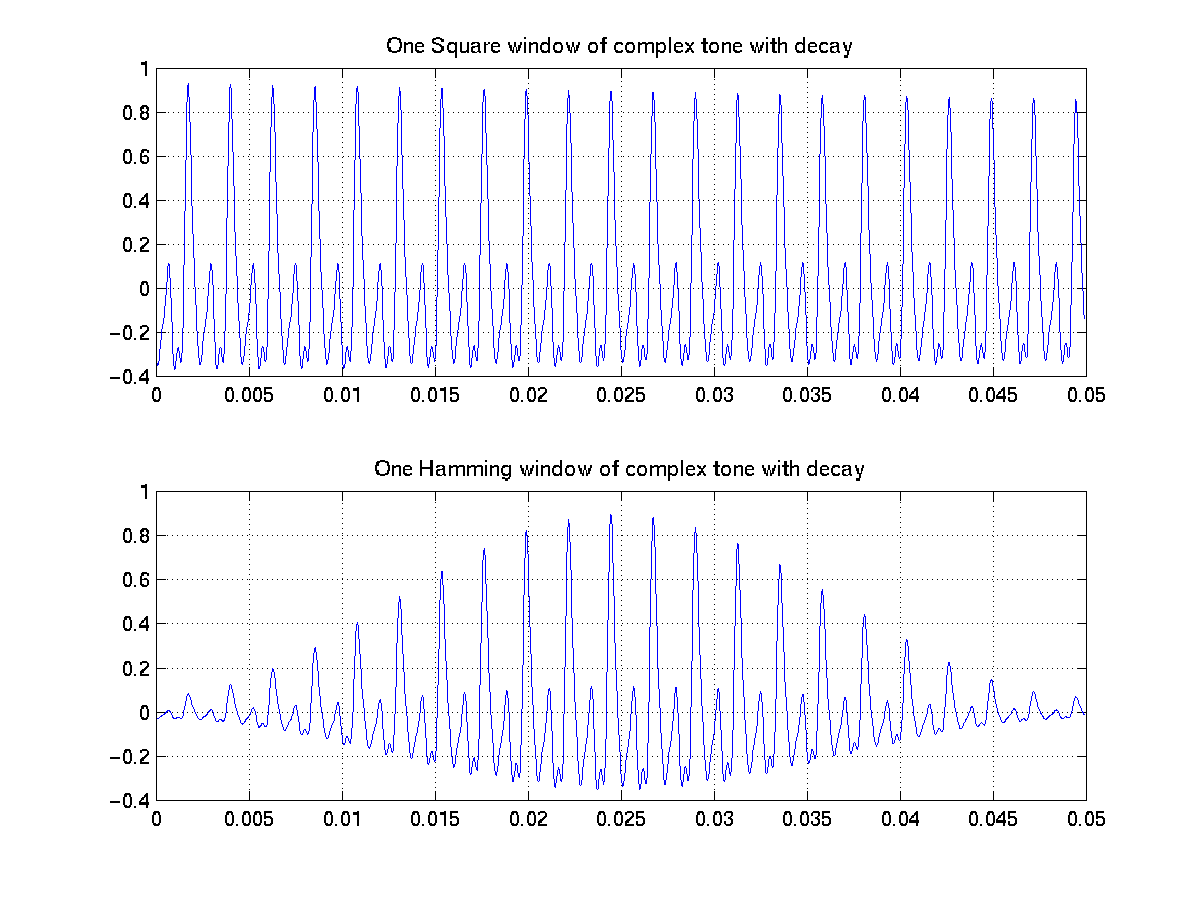
\includegraphics[width=120mm, height=70mm]{\HOME/figures/ComplexTone2200}
  }
  \caption{{\small A complex tone with frequencies 440, 880, 1320,
  1760, 2200 Hz and amplitudes that start at .3, .4, .1, .1, .08,
  (resp.), decaying exponentially. (top) a square window and (bottom) a
  Hamming window each of length 0.05 seconds.} }
  \label{fig:ComplexTone2200}
  %\end{figure}
  
  %\begin{figure}
  \ifthenelse{\boolean{nofigures}}{}{
    \centering  
    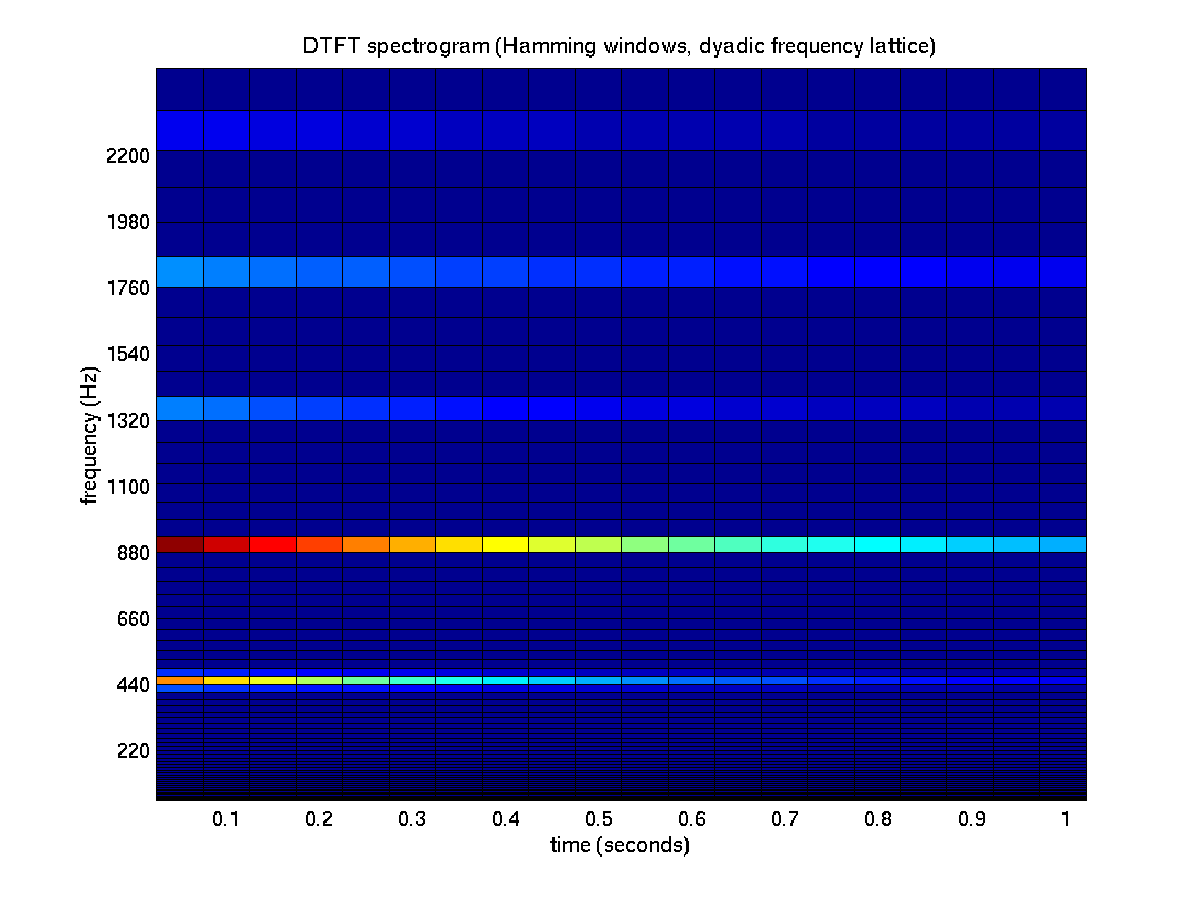
\includegraphics[width=120mm, height=70mm]{\HOME/figures/SpecDTFTHam2200}
  }
  \caption{{\small The DTFT of a complex tone with frequencies 440, 880, 1320,
  1760, 2200 Hz and amplitudes that start at .3, .4, .1, .1, .08,
  (resp.), decaying exponentially.  The time dimension is divided into
  0.05 second Hamming windows.  Amplitudes are computed along the
  frequency axis at the points $55 \cdot 2^{k/12}$ where $k=0, 1,
  \ldots, 96$.} }
  \label{fig:SpecDTFTHam2200}
\end{figure}
  
\begin{figure}
  \ifthenelse{\boolean{nofigures}}{}{
    \centering  
    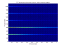
\includegraphics[width=120mm, height=70mm]{\HOME/figures/SpecFFTHam2200}
  }
  \caption{{\small The FFT of a complex tone with frequencies 440, 880,
  1320, 1760, 2200 Hz and amplitudes that start at .3, .4, .1, .1, .08,
  (resp.), decaying exponentially.  The time dimension is divided into
  0.05 second Hamming windows.  Amplitudes are computed along the
  frequency axis at 2200 evenly spaced frequencies.}}
  \label{fig:SpecFFTHam2200}
\end{figure}
% (end: insert file: SpectralEstimation.tex)

% (begin: insert file DissonanceEstimation.tex)
\subsection{Fourier Based Dissonance Estimation}
\label{sec:FourierDissonance}
Consider modeling the signal $f$ as the sum of partials,
\[
f(t) = \sum_j p_j(t)
\]
with $p_j(t) = a_j(t)\cos\phi_j(t)$ and 
$\phi_j(t)= \omega_jt+\phi_j$.
Measured in Hertz, the instantaneous frequencies of the partials are
$f_j  = \phi'_j(t)/2\pi$.
A measure of the sensory dissonance between two pure sinusoids, $p_j$
and $p_k$, can be based on the empirical research of Plomp and
Levelt~\cite{Plomp:1965} discussed earlier.  

At time $t_0$, assume that the values $f_j = \phi'_j(t_0)/2\pi$ and
$f_k = \phi'_k(t_0)/2\pi$ are known.  Then we define an
\emph{instantaneous dissonance} measure between the two partials as
follows: 
%\begin{eqnarray*}D[a_j(t_0)\cos\phi_j(t),a_k(t)\cos\phi_k(t)]\\
\[
D[p_j,p_k](t_0)= a_j(t_0)a_k(t_0)d(f_j,f_k)
\]
%\end{eqnarray*}
For the metric $d(\cdot,\cdot)$ we employ the parameterization of the
Plomp-Levelt curves given by Sethares~\cite{Sethares:1997},
\begin{equation}
\label{eqn:diss}
d(f_j,f_k) = e^{-b_1x} - e^{-b_2x}
\end{equation} 
where $x(t) = |f_j - f_k|/\min\{f_j,f_k\}$.  The constants
$b_1$ and $b_2$ determine the rate at which the dissonance curve rises
and falls. %~\cite{Plomp:1965},
Sethares performed a gradient minimization of the squared error between
the function~(\ref{eqn:diss}) and the averaged Plomp and
Levelt data.  This values $b_1 = 3.5$ and $b_2=5.57$ produce the best
fit. 

Next, we define the \emph{instantaneous dissonance}
of the signal $f$ at time $t_0$ as the sum
\begin{equation}
\label{eqn:instDiss}
Df(t_0)= \frac{1}{2}\sum_{j,k}a_j(t_0)a_k(t_0)d(f_j,f_k)
\end{equation}

Of course, in general we cannot assume that the amplitudes and
instantaneous frequencies are known.  However, we can approximate
these data by assuming them constant over the time support
%Heisenberg boxes 
of each windowed Fourier atom $g_{s,u,\xi}$.  This assumption permits a 
measure of dissonance at each window including time $t_0$ for which
$(t_0,\xi(t_0))$ is a ridge point.  We take this as our estimate of
the instantaneous dissonance over the time window containing $t_0$.
More precisely, let $W_{t_0}=[t_{-},t_{+}]$ be the window containing
$t_0$.  At each ridge 
point $(t_0,\xi_j(t_0))$, with $t_0\in W_{t_0}$, we estimate 
\[
\tilde{f}_j = \xi_j(t_0)/2\pi, \qquad %\text{ and }\quad
\tilde{a}_j = \frac{2|Sf(t_0,\xi_j(t_0)|}{\sqrt{s}|\hat{g}(0)|}
\]
We take as our estimated sensory dissonance over the interval
$t \in W_{t_0}$ 
\begin{equation}
\label{eqn:estDiss}
\tilde{D}f(t)= 
\frac{1}{2}\sum_{j,k}\tilde{a}_j\tilde{a}_k d(\tilde{f}_j,\tilde{f}_k)
\end{equation}

\begin{figure}
  \ifthenelse{\boolean{nofigures}}{}{
    \centering  
    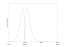
\includegraphics[width=120mm, height=70mm]{\HOME/figures/analyticDiss}
  }
  \caption{The exact dissonance curve computed with \emph{a priori}
  knowledge of the amplitudes and frequencies.  The horizontal axis
  delimits time, though the tick marks indicate the frequency of the
  linear tone.} 
  \label{fig:analyticDiss}
%\end{figure}

%\begin{figure}
  \ifthenelse{\boolean{nofigures}}{}{
    \centering  
    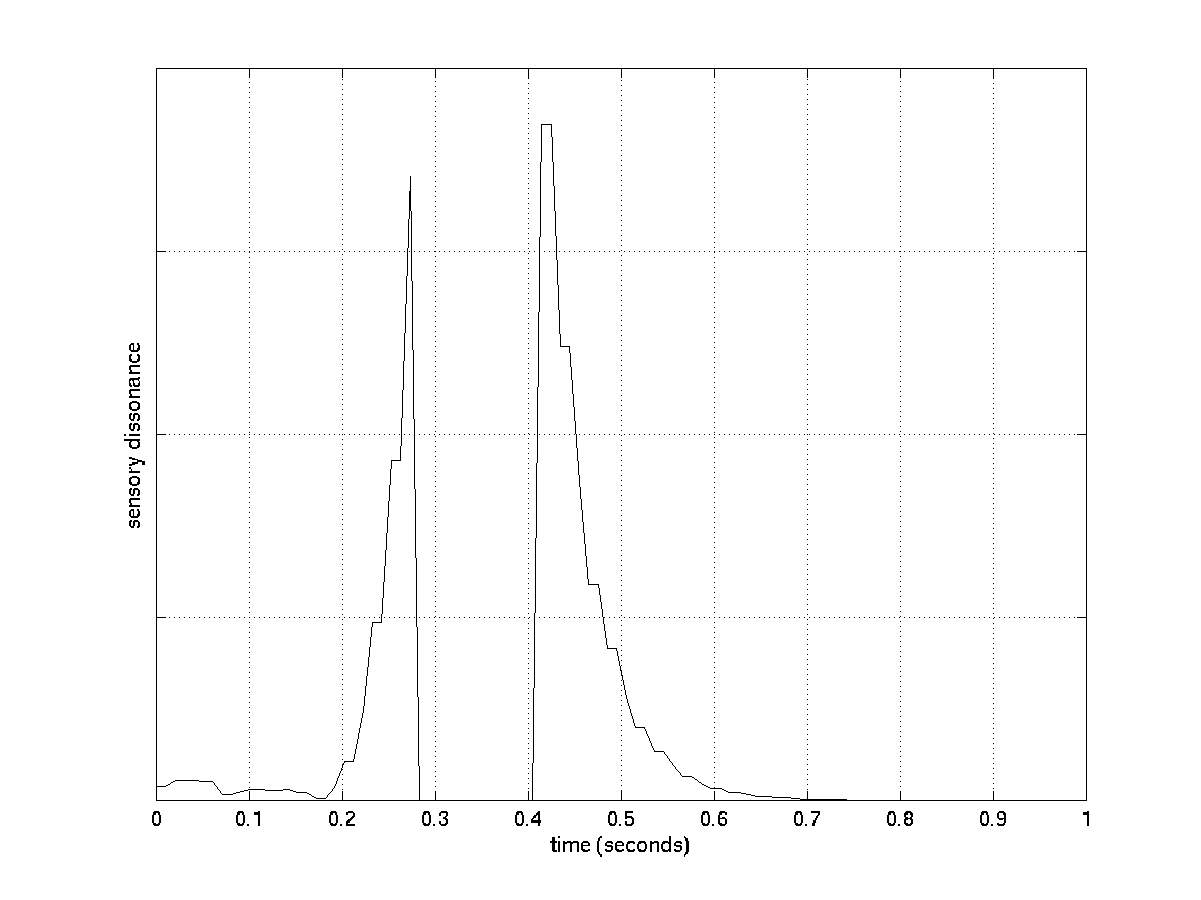
\includegraphics[width=120mm, height=70mm]{\HOME/figures/empiricalDiss}
  }
  \caption{The estimated dissonance curve computed with 
  ridge point estimates of amplitudes and frequencies.}
  \label{fig:empiricalDiss}
\end{figure}

Figure~\ref{fig:analyticDiss} shows the instantaneous dissonance of
the signal~(\ref{eqn:purelin440}) as $t$ varies over $[0,1]$.  It is
computed using~(\ref{eqn:instDiss}).  Figure~\ref{fig:empiricalDiss}
shows the estimated dissonance of the same signal.  It is computed
by taking amplitude and frequency estimates from the ridges in
Figure~\ref{fig:ridges} and plugging them into~(\ref{eqn:estDiss}).
As we can see, the windowed Fourier atoms do not provide a high enough
frequency resolution to provide a reliable dissonance measure on the
interval $t\in[.3,.4]$.  This corresponds to a frequency interval
for the linear chirp of about $[418, 484]$ Hz.  
For a musical
%If this were a musical 
signal, this implies that only frequency intervals of more than 2
semitones are distinguishable.  One might argue that, for a method to
be useful for musical applications, it must be able to discriminate 
between two components that are one semitone apart.  
%This provides a
%clear objective for future work, and a criteria by which such work
%may be judged. 
% (end: insert file DissonanceEstimation.tex)

\subsection{Matching Pursuit}
\label{sec:Practical-MP}
This section describes how we implement the atomic decomposition
of a signal using the matching pursuit algorithm described in
section~\ref{sec:MP}.  

The Matlab program {\tt MZMP.m}, appearing in section~\ref{sec:MZMP},
computes the optimal gabor atoms for representing a given signal.  
The primary sub-routines it calls are {\tt gaborMZ.m} and {\tt IP.m},
which listed in sections~\ref{sec:gaborMZ} and~\ref{sec:IP},
respectively.  The {\tt gaborMZ} sub-routine computes individual
gabor atoms given a set of parameters.  (Section~\ref{sec:MP}
describes the parameters that define a gabor atom.)  The {\tt IP}
sub-routine computes the inner product of two gabor atoms from
their given parameters without actually constructing the atoms.

\subsection{Energy Separation}
\label{sec:Practical-energy-separation}
This section describes the implementation of the energy separation
technique described in section~\ref{sec:energy-separation}.

The Matlab program {\tt DEnergy.m} appears in
section~\ref{sec:DEnergy}, and computes the \emph{signal energy}
and \emph{interference energy} of a given signal.  (The italicized
terms are defined in section~\ref{sec:energy-separation}.)  The first
step in this process is a call to the {\tt MZMP} routine, which
computes the matching pursuit decomposition of the signal. The output
of {\tt MZMP} are the parameters of a collection of gabor atoms
which optimally represent the given signal. Next, the Wigner and
cross-Wigner transforms of these optimal atoms are computed by calling
the sub-routines {\tt WVTrans\_AF.m} and {\tt WVTrans\_AFC.m},
respectively.  Finally, the {\tt DEnergy} routine (optionally)
produces a time-frequency display of the signal energy and
interference energies.

\subsection{Energy Based Dissonance Estimation}
\label{sec:EnergyDissonance}
